
\section{Methodology of Systematic Survey}
\subsection{Sources of Information}
In this paper, we conducted an empirical study following \cite{keele2007guidelines,petersen2015guidelines}. The purpose of this study is to collect and examine papers from the year 2011 to 2022 focusing on vulnerability detection across various programming languages and source codes using machine learning and deep learning techniques. The period between 2011 and 2022 is an appropriate time interval for reviewing data-driven vulnerability detection for several reasons: 
a) {\textbf{Increase in the volume and diversity of software vulnerabilities}: Over the past decade, there has been a significant increase in the number and diversity of software vulnerabilities that have been discovered and reported~\footnote{https://nvd.nist.gov/general/news}. As of 2021, there exist 150,000 CVE records in the National Vulnerability Database (NVD)\footnote{https://nvd.nist.gov/general/brief-history}. This increase has created a need for more sophisticated and effective methods for vulnerability detection, which has led to the development of new data-driven techniques.
b) \textbf{Advancements in ML/DL and data analytics}: The past decade has seen significant advancements in machine learning, including the development of deep learning algorithms~\cite{goodfellow2020generative, hinton2006fast}, natural language processing techniques~\cite{devlin2018bert, liu2019roberta}, and other data-driven approaches that are highly effective in detecting software vulnerabilities.

While we start collecting papers, we search for relevant research papers from four available databases, which are ScienceDirect, IEEE Xplore, ACM digital library, and Google Scholar. 
\subsection{Search Terms}
%\jie{Unclear about the relations among the keywords in the box below, should use `add' `or' to specify the relation.}\nima{This comment is confusing for me.} \song{Nima: how you connect these keywords when combine them in the search engine? "or" or "and"} \nima{I used "or"}
From earlier work, we identify key phrases used in the search~\cite{le2021survey,lin2020software,zeng2020software,semasaba2020literature} and our experience with the subject area. The following are the search terms: 


\noindent\fbox{%
\parbox{\textwidth}{\textit{vulnerability detection} \textcolor{red}{OR} \textit{security vulnerability detection} \textcolor{red}{OR}
\textit{vulnerability detection using machine learning} \textcolor{red}{OR} \textit{vulnerability detection using deep learning} \textcolor{red}{OR} 
\textit{source code security bug prediction} \textcolor{red}{OR} \textit{source code vulnerability detection} \textcolor{red}{OR} \textit{source code bug prediction}}}

\subsection{Study Selection}
The process of selecting studies to be included in our survey involves the following stages: (1) initially choosing studies based on their title, (2) selecting studies after reviewing their abstracts, and (3) making further selections after reading the full papers. Note that, the initial search results contain entries that are not related to security vulnerability detection. This might be caused by accidental keyword matching. We manually check each paper and remove these irrelevant papers to ensure the quality of our survey dataset. We also observe that there exist duplicate papers among search results  since the same study could be indexed by multiple databases. We then discarded duplicate studies manually. 
To assist the selection of papers that have presented new ML or DL-based models for software vulnerability identification, we provide the following inclusion and exclusion criteria:
\begin{itemize}
\item The studies should have been peer-reviewed 
    \item The studies should have experimental results
    \item The studies should employ an ML or DL technique
    \item The studies improve existing data-driven vulnerability detection techniques
    \item The input to ML/DL models should be either source code, commit, or byte-codes
\end{itemize}

Also, we have the following exclusion criteria to filter out irrelevant papers:

\begin{itemize}
    \item Studies focusing on other engineering domains
    \item Studies addressing static analysis, dynamic analysis, mutation testing, fault localization
    \item Review papers
    \item Studies focusing on vulnerability detection of web and Android applications
    \item Studies belonging to one of the following categories: books, chapters, tutorials, technical reports
    \item Studies using code similarity or clone detection tools
    \item Studies focusing on malware detection on mobile devices, intrusion detection, and bug detection using static code attributes
\end{itemize}

Using these criteria, we narrow down our findings by examining each paper's title, abstract, and contents to get the most relevant and high-quality research papers. To make human effort manageable, we developed a script to automatically get high-quality records close to the software vulnerability detection problem. To summarize, in the first stage, we began with a total of 3,154 papers obtained from the database search. From this initial pool, 880 papers were chosen for further evaluation in the second stage. During the second stage, these papers were reviewed based on their abstracts, resulting in the selection of 116 papers with relevant abstracts. Finally, in the third stage, after reading the full papers, 67 papers were ultimately chosen for inclusion in the study. %{We have manully checked that all 75 papers we selected to address our research questions meet our inclusion and exclusion criteria and are closely related to detecting software vulnerabilities. To improve the quality of the papers, we also checked the ranking in the core conference ranking forum\footnote{http://portal.core.edu.au/conf-ranks} and only included papers with a ranking of \textit{B} or higher which resulted in 67 primary papers to address research questions.}

\subsection{Study Quality Assessment}
\label{sec:squality}
% \song{fill this section} \nima{to be done}
For each of the final selected studies, we answered the questions below to assess its quality:
\begin{itemize}
\item Is there a clearly stated research goal related to software vulnerability detection? 
\item Is the proposed vulnerability detection approach used ML or DL techniques?
\item Is there a defined and repeatable technique?
\item Is there any explicit contribution to vulnerability detection?
\item Is there a clear methodology for validating the technique?
\item Are the subject projects selected for validation suitable for the research goals?
\item Are there control techniques or baselines to demonstrate the effectiveness of the vulnerability detection technique?
\item Are the evaluation metrics relevant (e.g., evaluate the effectiveness of the proposed technique) to the research objectives? 
\item Do the results presented in the study align with the research objectives and are they presented in a clear and relevant manner?
 \end{itemize}   

%\jie{Do we need to specify the quality status or quality score distribution of the collected studies?}\nima{What is score distribution?} \song{Nima: check section 2.1.5: https://www.eecs.yorku.ca/~wangsong/papers/esem18.pdf}
% Each question has three possible responses and associated numerical values, i.e., yes (1), no (0), or somewhat (0.5). 
% The sum of responses to the quality assessment questions provides a relative
% measure of study quality. The average quality score was 8.5, which indicates the high quality of the selected studies.

\subsection{Selection Verification}
\label{sec:sverification}
The process of creating a taxonomy for the selected 67 primary studies involves several steps. Initially, the lead author establishes a preliminary taxonomy that groups the studies together based on their research questions. This taxonomy provides a basic framework for organizing the studies in a meaningful and systematic manner. Next, the lead author expands the taxonomy by assigning new papers to the preliminary taxonomy. If a new paper cannot fit into any of the existing categories within the taxonomy, a new category is created that reflects the unique characteristics of that paper. To ensure the accuracy of the taxonomy, the second and third authors (who are not involved in the taxonomy creation process) randomly select 20 papers from the workflow and check the created taxonomies for any discrepancies. They then mark any disagreements they find, and all three authors discuss and resolve these disagreements. Initially, the disagreement rate was 30\%, but after a second round of review and cross-checking of the papers, the authors were able to eliminate all disagreements.

% \song{fill this section}

% The first author did the selection of the studies following the process outlined before. 
% The second author provided validation of the studies at each stage of the selection process. After stage 1, 10\% of the studies were randomly selected for the second author to validate. The first author prepared the selection, ensuring that the sample had approximately the same proportion of selected and rejected studies as the full population. Results show that 95\% of the studies had the same selection by the first and second author. All the differences were between the studies the first author selected but the second author did not. The discrepancy is caused by the differences between the interpretations of the scope of software vulnerability and ML or DL-based approaches. However, we found that all these papers were not included in the final set, so it did not influence the results. After stage 2, the second author evaluated the abstracts for 10\% randomly selected studies. We again ensured that the sample had approximately same distribution of selected and rejected studies as the full population of studies. 96\% of the randomly selected studies have the same classification by the two authors. Similarly
% with stage 1, most of the differences came from these studies the first author classified as “1” but the second author classified as “0”. It is worth mentioning that these papers were not included in the final set. We also conducted similar selection verification process for stage 3, and all the randomly selected studies 20\% have the same selection by the two authors.




\begin{figure}[t!]
    \centering
     {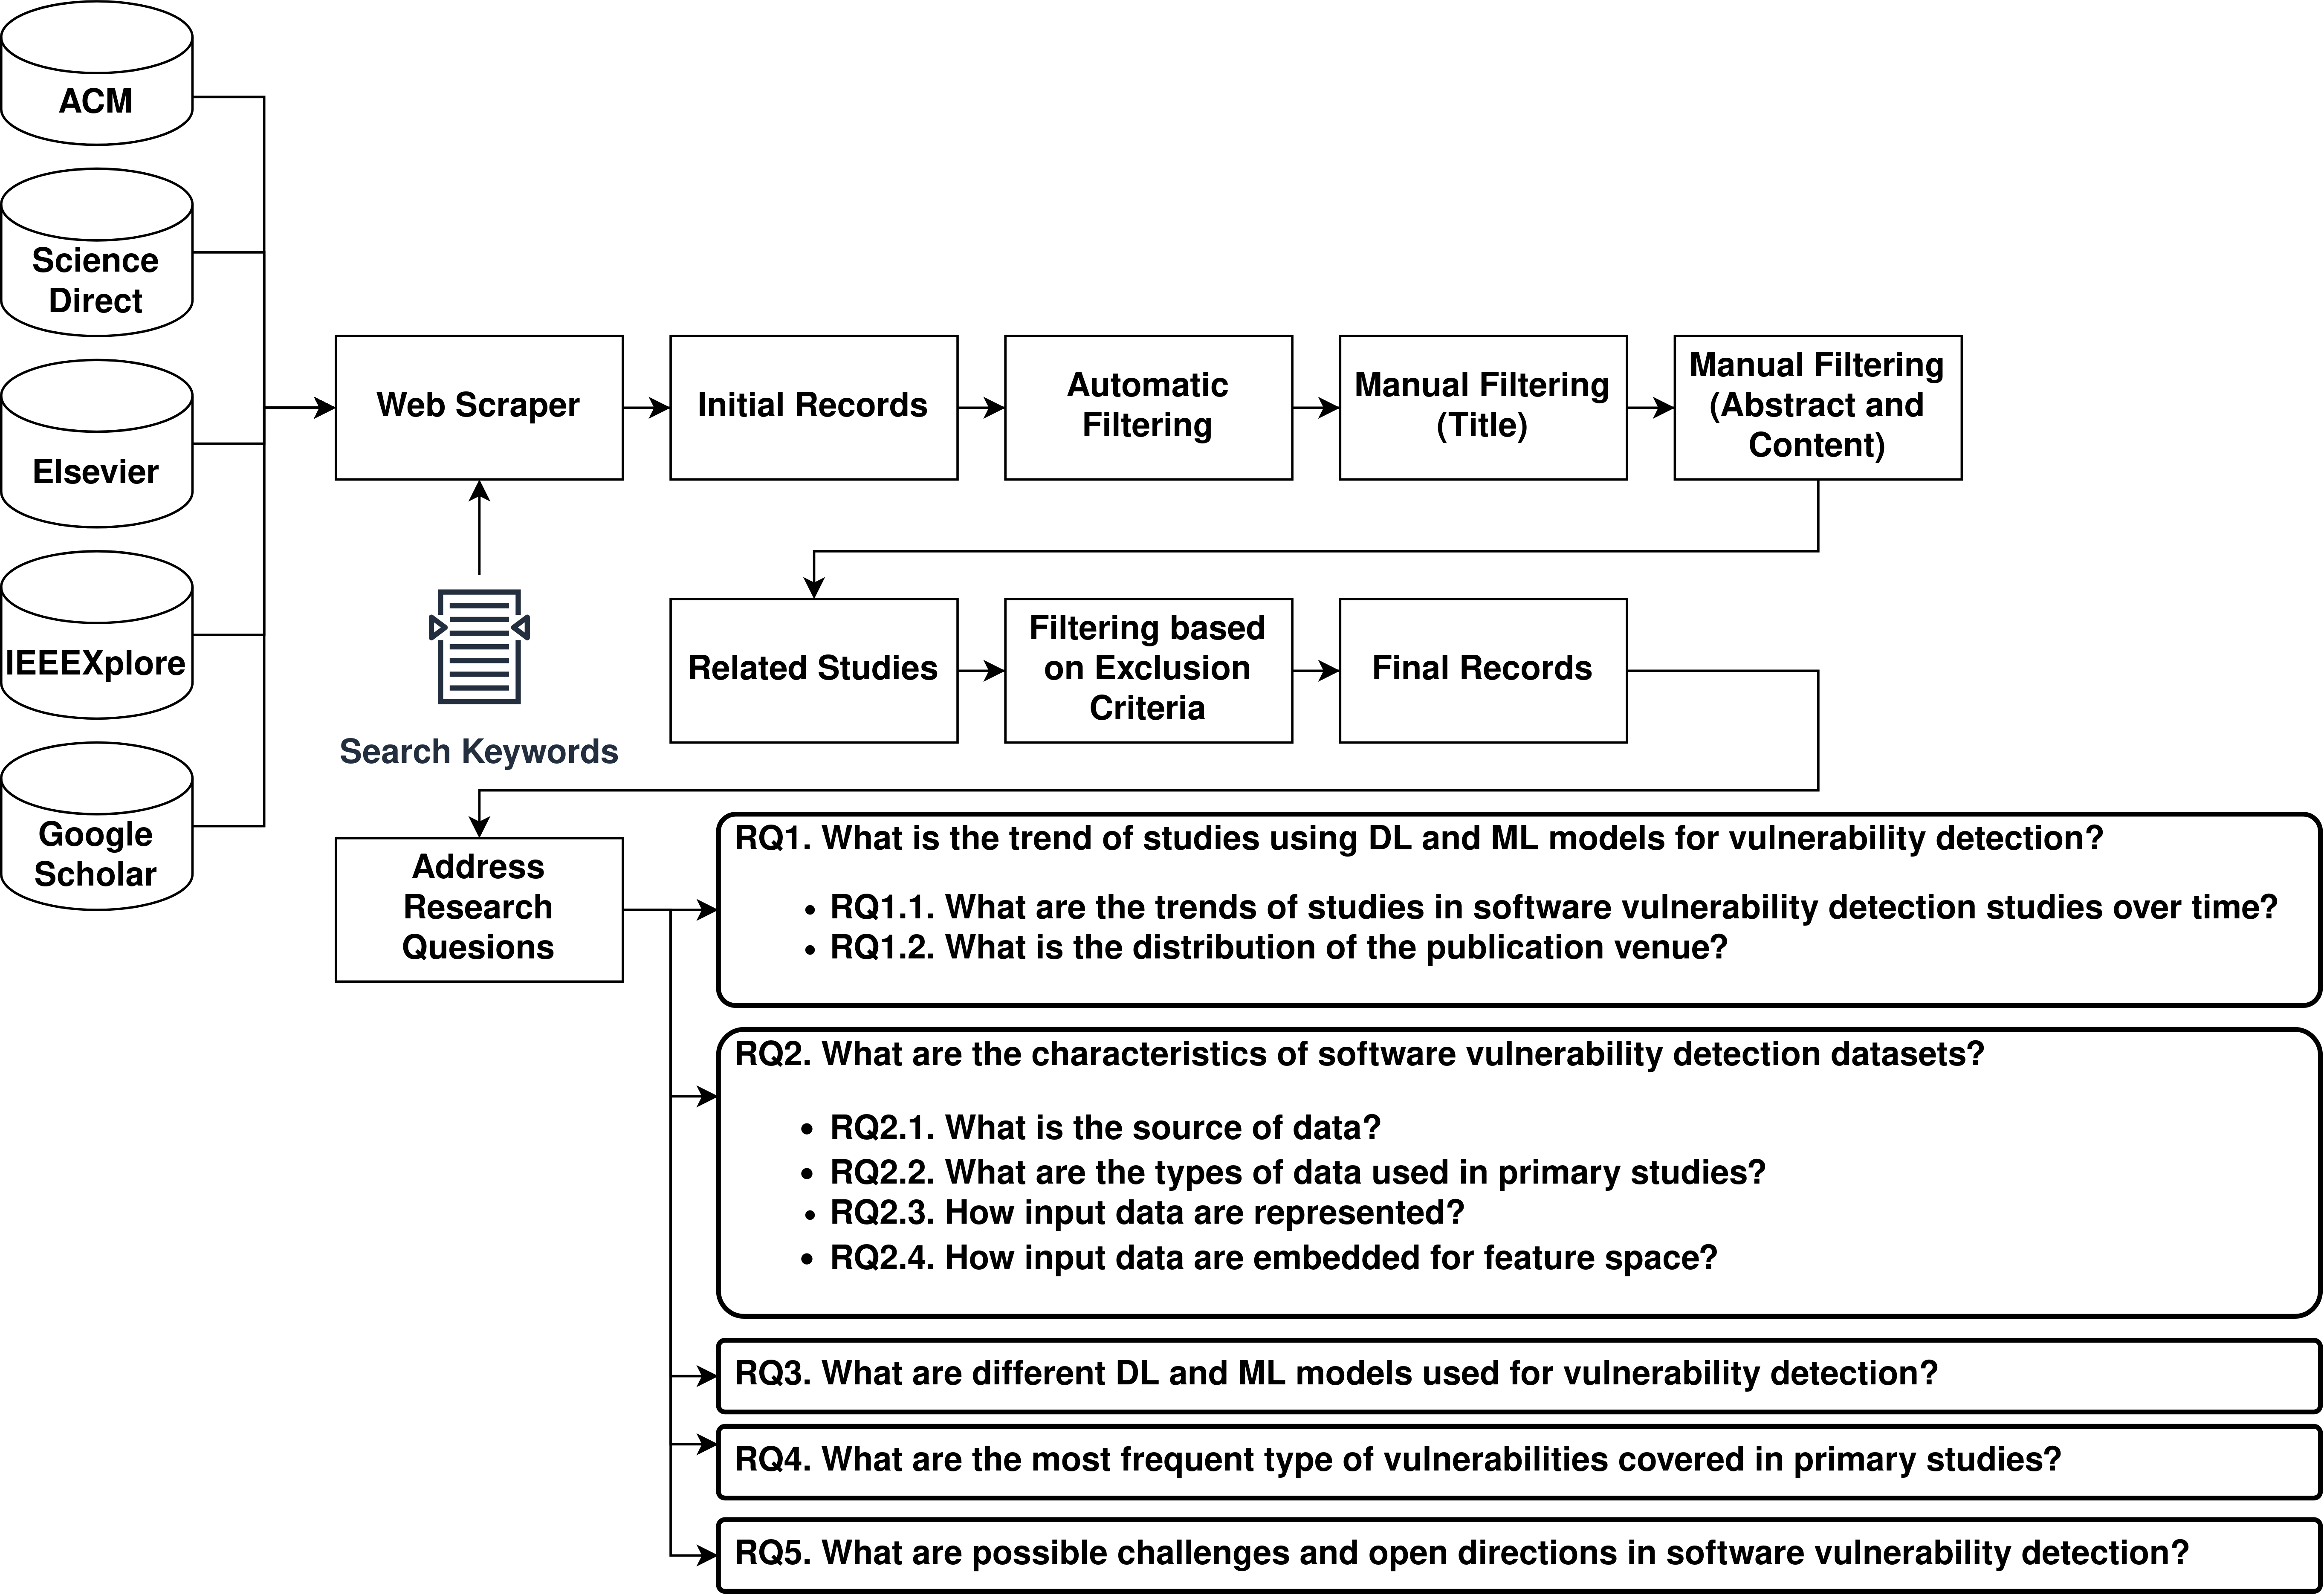
\includegraphics[width=1\textwidth]{Figures/flow.png}}\
     %\vspace{-0.1in}
     \caption{The workflow of our survey.}
    \label{vuldiag}
\end{figure}

